\section{Using Adaptivity and Local Refinement}

\subsection{Adaptivity in general}

\subsubsection*{What is adaptivity all about?}

\begin{frame}
  \frametitle<presentation>{What is adaptivity all about?}
  \begin{center}
    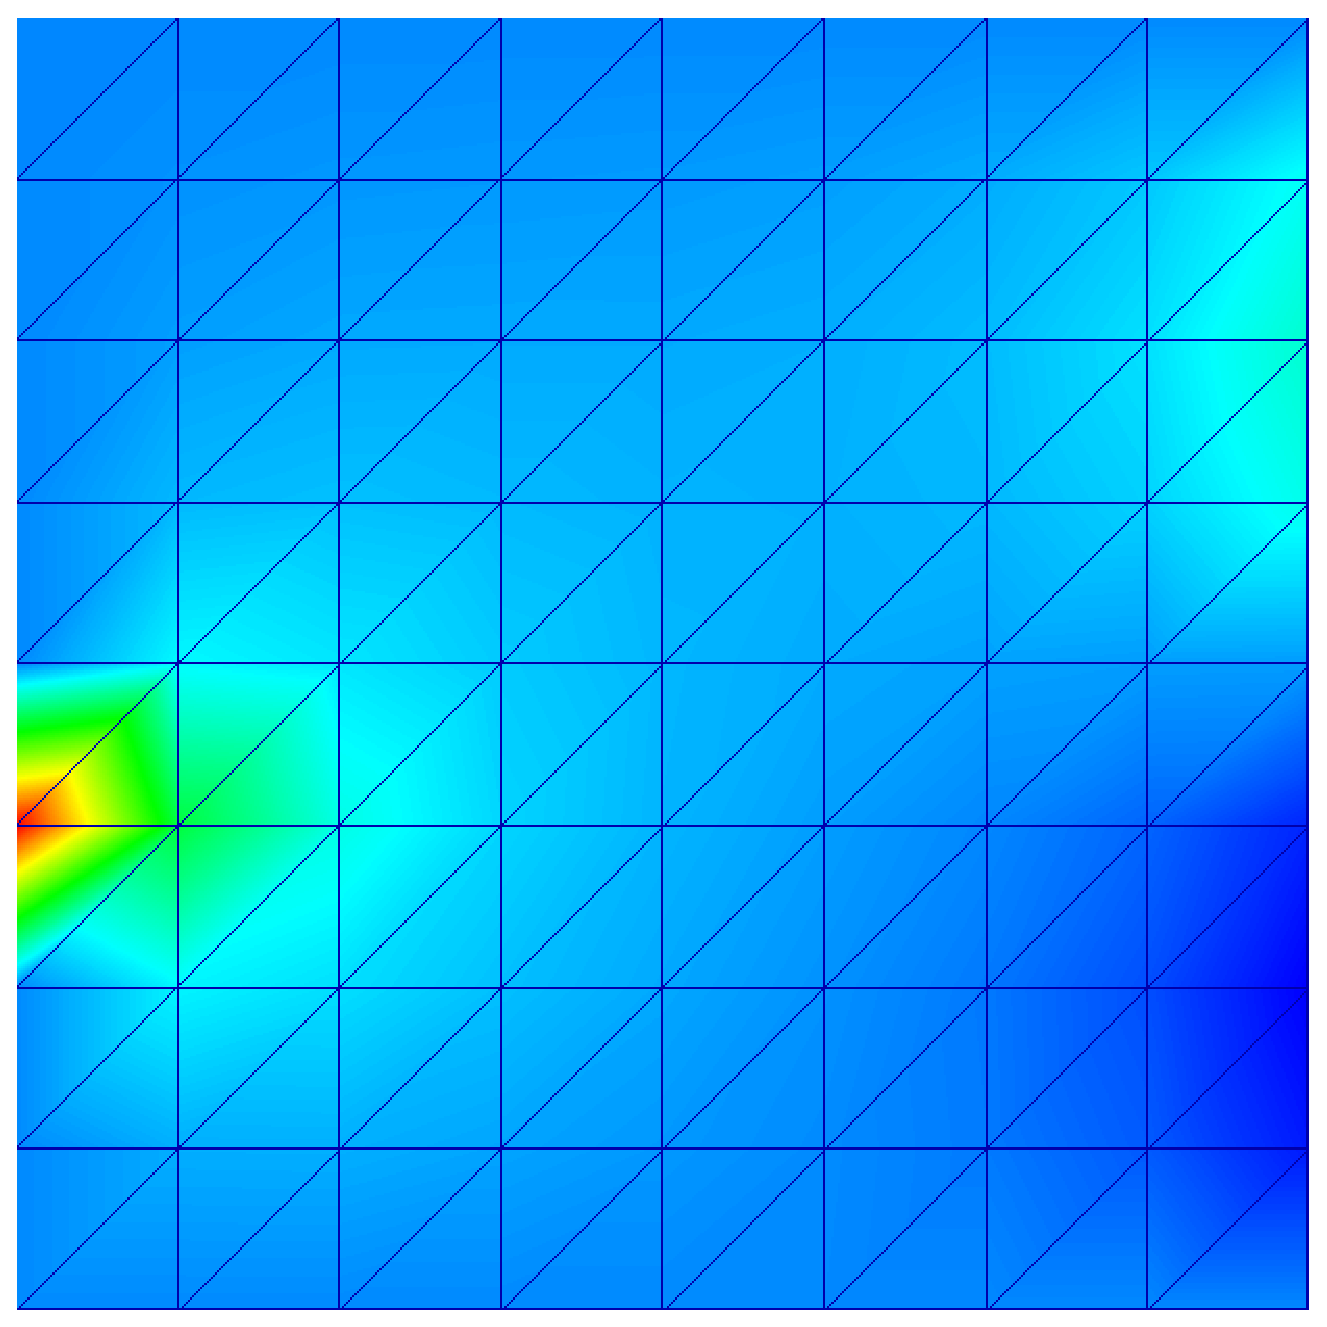
\includegraphics[width=0.4\textwidth]{EPS/adaptivity/low_resolution}

    A coarse discretisation may not be able to capture \\ all the features of the solution \ldots

    \begin{tabular}{rl}
      $h$:          & $2^{-3}$ \\
      DOF:          & 81       \\
      Time (total): & 0.026 s
    \end{tabular}
  \end{center}
\end{frame}

\begin{frame}
  \frametitle<presentation>{What is adaptivity all about?}
  \begin{center}
    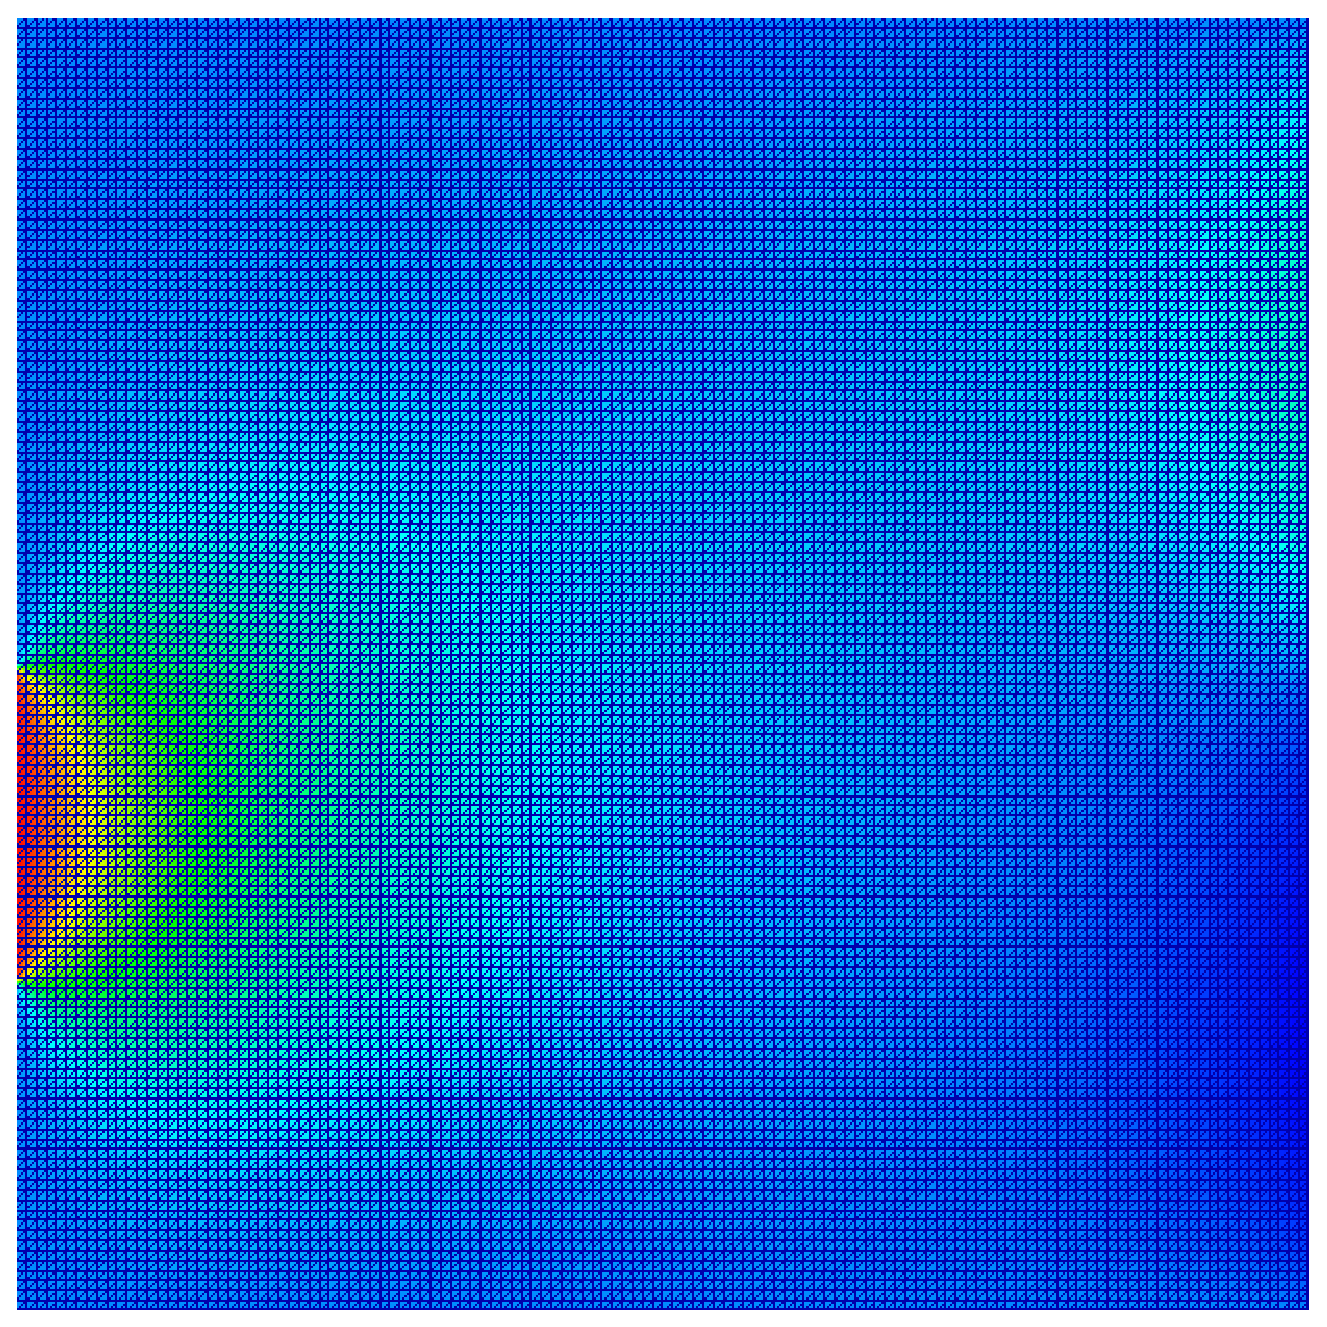
\includegraphics[width=0.4\textwidth]{EPS/adaptivity/high_resolution}

    \ldots while a fine discretisation may have \\ too many degrees of freedom to be feasable.

    \begin{tabular}{rl}
      $h$:          & $2^{-7}$ \\
      DOF:          & 16641    \\
      Time (total): & 38.3 s
    \end{tabular}
  \end{center}
\end{frame}

\begin{frame}<presentation>
  \frametitle<presentation>{What is adaptivity all about?}
  \begin{center}

    \only<1>{
    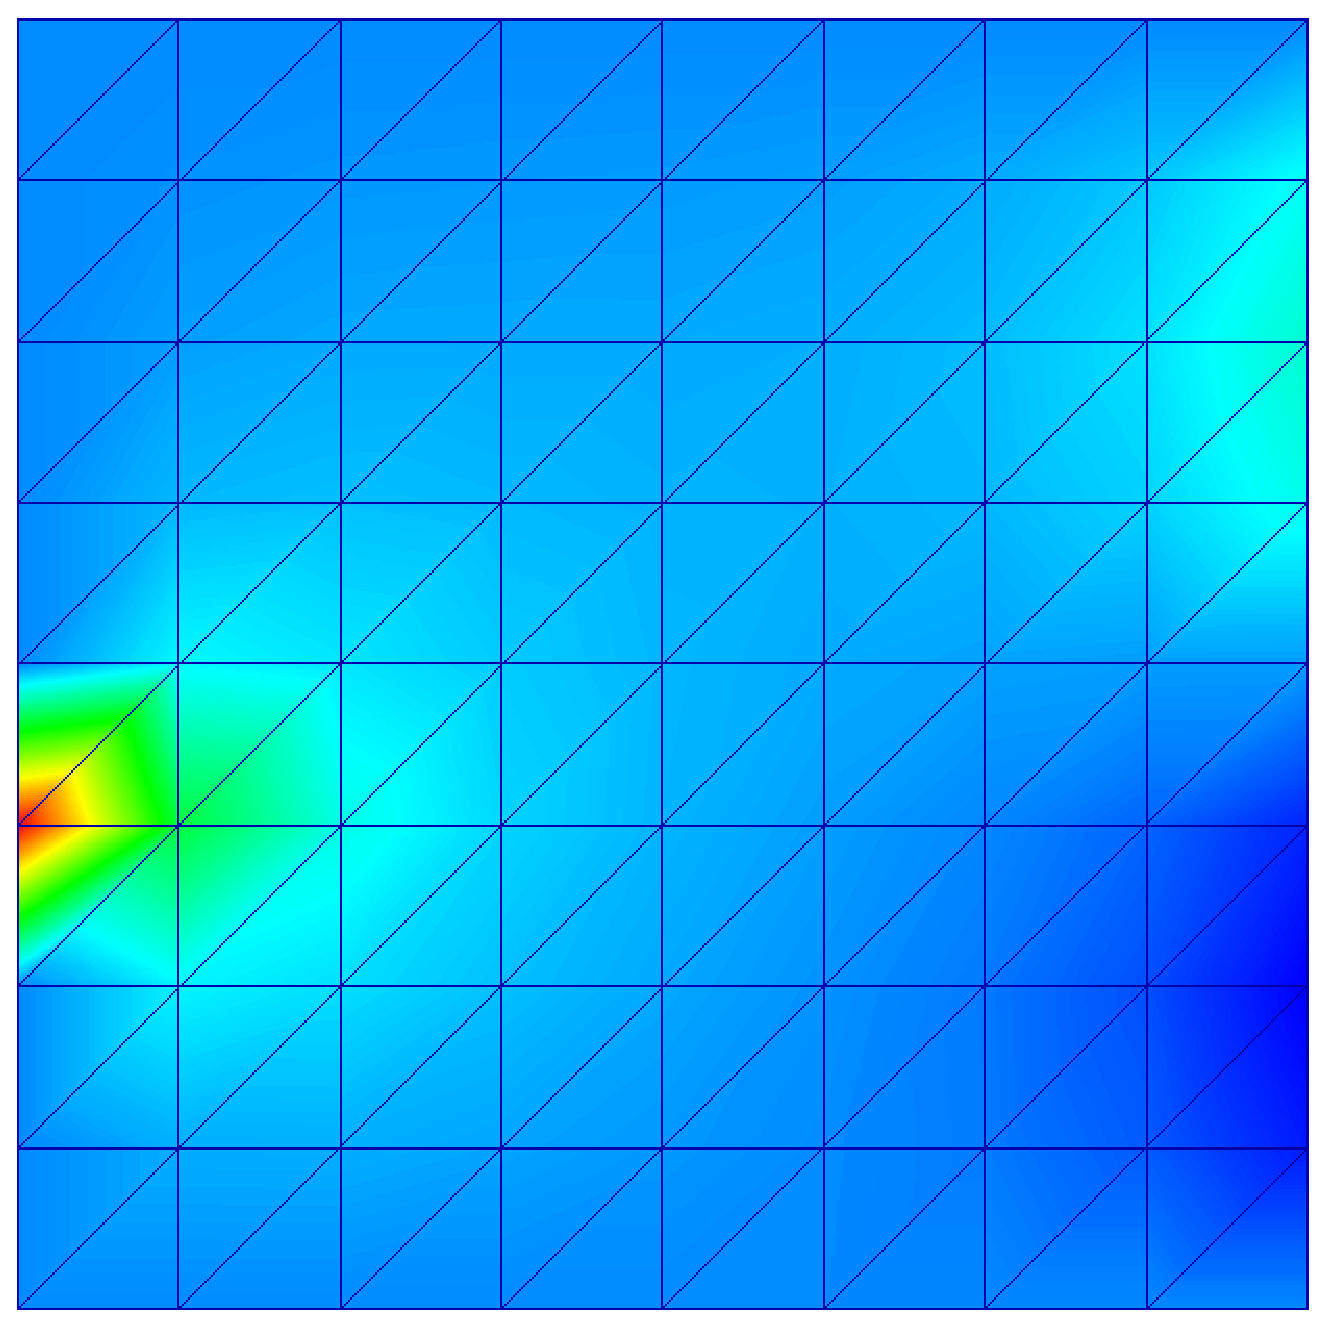
\includegraphics[width=0.4\textwidth]{EPS/adaptivity/adaptivity1}
    }

    \only<2>{
    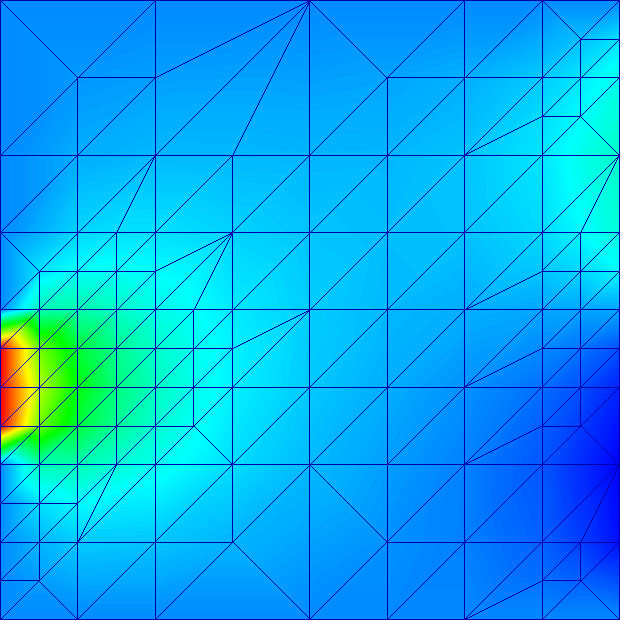
\includegraphics[width=0.4\textwidth]{EPS/adaptivity/adaptivity2}
    }

    \only<3>{
    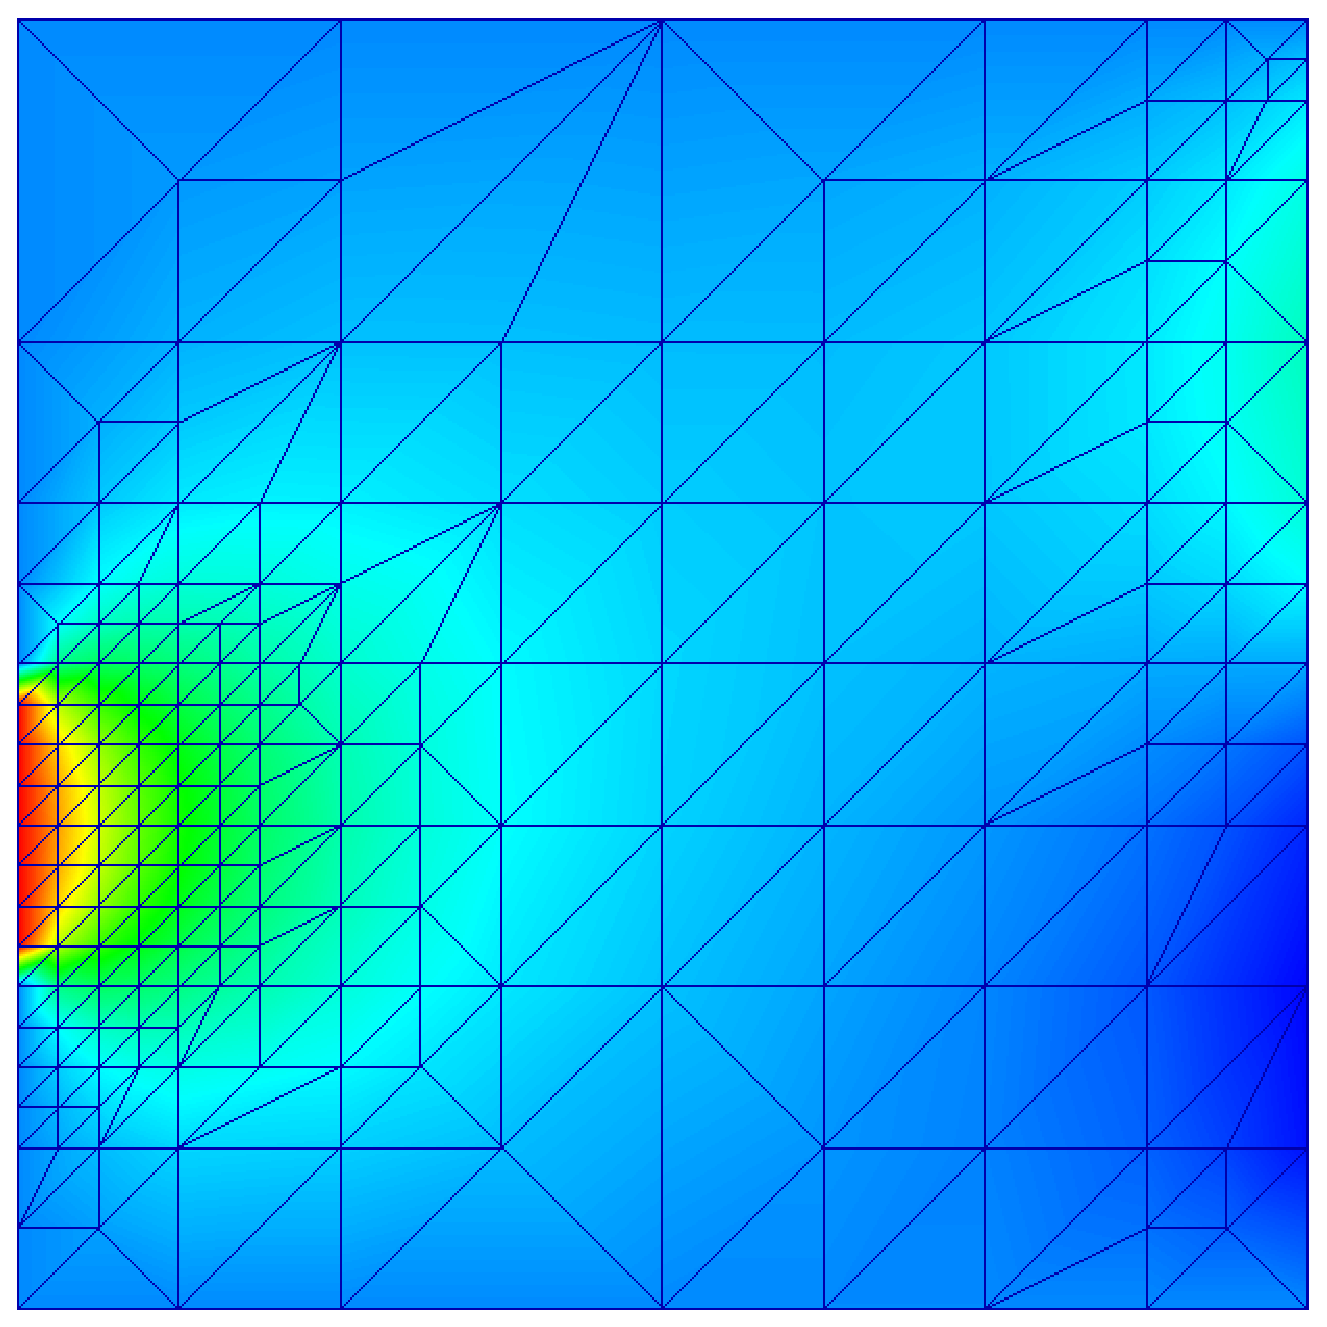
\includegraphics[width=0.4\textwidth]{EPS/adaptivity/adaptivity3}
    }

    \only<4>{
    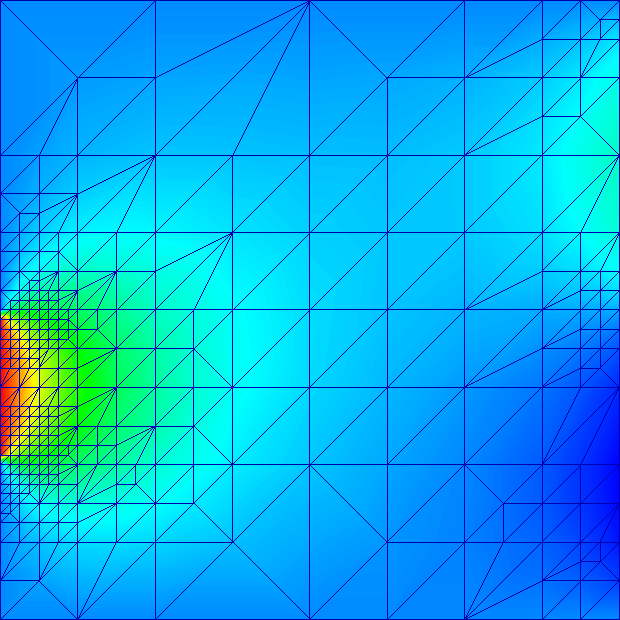
\includegraphics[width=0.4\textwidth]{EPS/adaptivity/adaptivity4}
    }

    \only<5>{
    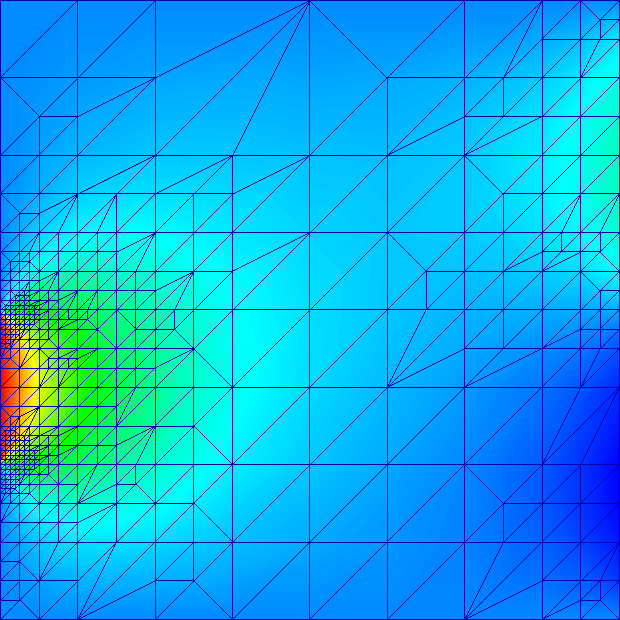
\includegraphics[width=0.4\textwidth]{EPS/adaptivity/adaptivity5}
    }

    \emph{Idea:} Use a higher resolution only in areas where it is beneficial.

    \only<1>{
    \begin{tabular*}{0.95\textwidth}{rl}
      $h_{\min}$:   & $2^{-3}$ \\ 
      DOF:          & 81       \\
      Time (total): & 0.026s
    \end{tabular*}
    }

    \only<2>{
    \begin{tabular*}{0.95\textwidth}{rl}
      $h_{\min}$:   & $2^{-4}$                         \\
      DOF:          & 81 + 124        = \alert{205}    \\
      Time (total): & 0.026s + 0.059s = \alert{0.085s}
    \end{tabular*}
    }

    \only<3>{
    \begin{tabular*}{0.95\textwidth}{rl}
      $h_{\min}$:   & $2^{-5}$                                  \\
      DOF:          & 81 + 124 + 200           = \alert{405}    \\
      Time (total): & 0.026s + 0.059s + 0.090s = \alert{0.175s}
    \end{tabular*}
    }

    \only<4>{
    \begin{tabular*}{0.95\textwidth}{rl}
      $h_{\min}$:   & $2^{-6}$                                          \\
      DOF:          & 81 + 124 + 200 + 323             = \alert{728}    \\
      Time (total): & 0.026s + 0.059s + 0.090s + 0.15s = \alert{0.325s}
    \end{tabular*}
    }

    \only<5>{
    \begin{tabular*}{0.95\textwidth}{rl}
      $h_{\min}$:   & $2^{-7}$                                                  \\
      DOF:          & 81 + 124 + 200 + 323 + 506               = \alert{1234}   \\
      Time (total): & 0.026s + 0.059s + 0.090s + 0.15s + 0.27s = \alert{0.595s}
    \end{tabular*}
    }

  \end{center}
\end{frame}

\begin{frame}<article>
  \begin{center}

    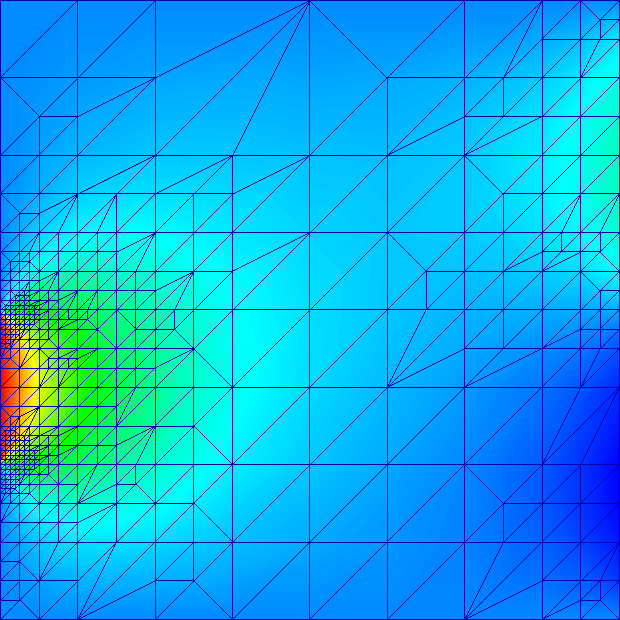
\includegraphics[width=0.4\textwidth]{EPS/adaptivity/adaptivity5}

    \emph{Idea:} Use a higher resolution only in areas where it is beneficial.

    \begin{tabular*}{0.95\textwidth}{rl}
      $h_{\min}$:   & $2^{-7}$                                                  \\
      DOF:          & 81 + 124 + 200 + 323 + 506               = \alert{1234}   \\
      Time (total): & 0.026s + 0.059s + 0.090s + 0.15s + 0.27s = \alert{0.595s}
    \end{tabular*}

  \end{center}
\end{frame}

\begin{frame}
  \frametitle<presentation>{What is adaptivity all about?}
  \begin{center}
    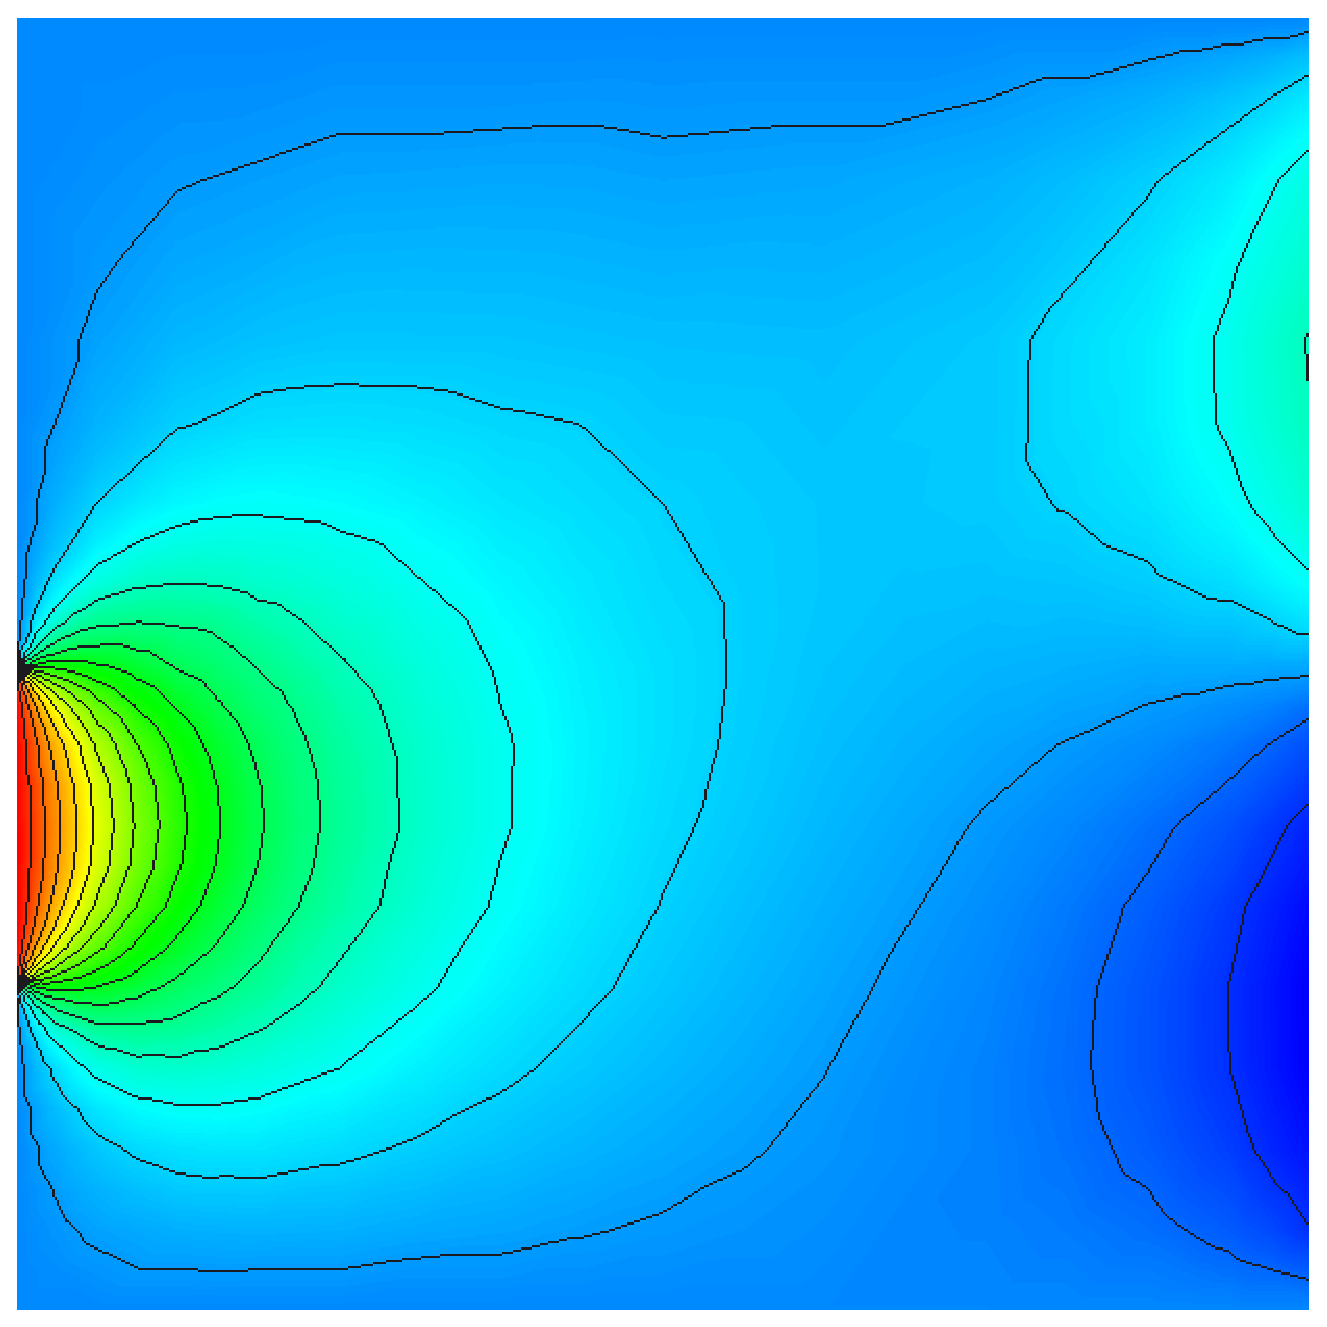
\includegraphics[width=.45\textwidth]{EPS/adaptivity/adaptive_iso} \hfill
    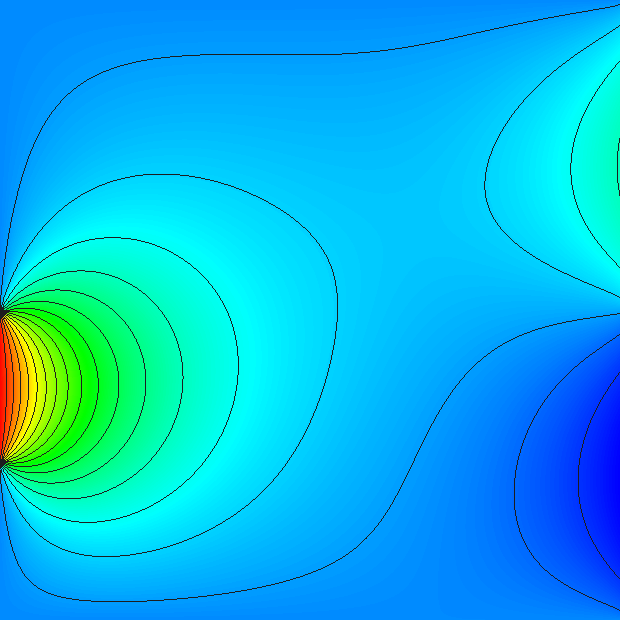
\includegraphics[width=.45\textwidth]{EPS/adaptivity/fine_iso}

    Adaptive     \hfill \hspace{7ex}Local refinement may lead to   \hfill Globally refined

    506 DOFs     \hfill \hspace{3ex}similar results using far less \hfill 16641 DOFs

    \alert{0.6s} \hfill computational effort.                      \hfill \alert{38s}

  \end{center}
\end{frame}

\begin{frame}
  \frametitle<presentation>{What is adaptivity all about?} 

  Adaptive Scheme
  \[
  (\mathbb{T}_n,C_{n}) \stackrel{\nu_n}{\rightarrow} (\mathbb{T}_{n+1},C_{n+1})
  \]

  Combined with \emph{error control}, adaptivity aims for optimization of the computational effort with a constraint on the maximum tolerated discretization error.

  \begin{block}{Adaptation goals}
    \begin{itemize}
      \item enhance accuracy in a localized manner
      \item reduce cost of the simulation.
    \end{itemize}
  \end{block}
\end{frame}

\begin{frame}
  \frametitle<presentation>{What is adaptivity all about?}
  \begin{block}{\emph{Main Problem}}
    How do we decide which regions are to be refined?

    It would be best to e.g.~spread the discretisation error evenly over the domain.
  \end{block}

  \pause
  \begin{block}{\emph{Solution}}
    Implement an \emph{\emph{error estimator}} with local \emph{\emph{error indicators}} computing a rough estimate of the discretisation error and refine regions with high local error.
  \end{block}

  Error estimators are taylored to the problem at hand, and the creation of \emph{efficient} error estimators is an active area of research.
\end{frame}

\begin{frame}[fragile]
  \frametitle<presentation>{Error Indication}

  \begin{center}
    \begin{minipage}{0.75\textwidth}
      \begin{center}
        Error indication by maximal concentration difference

        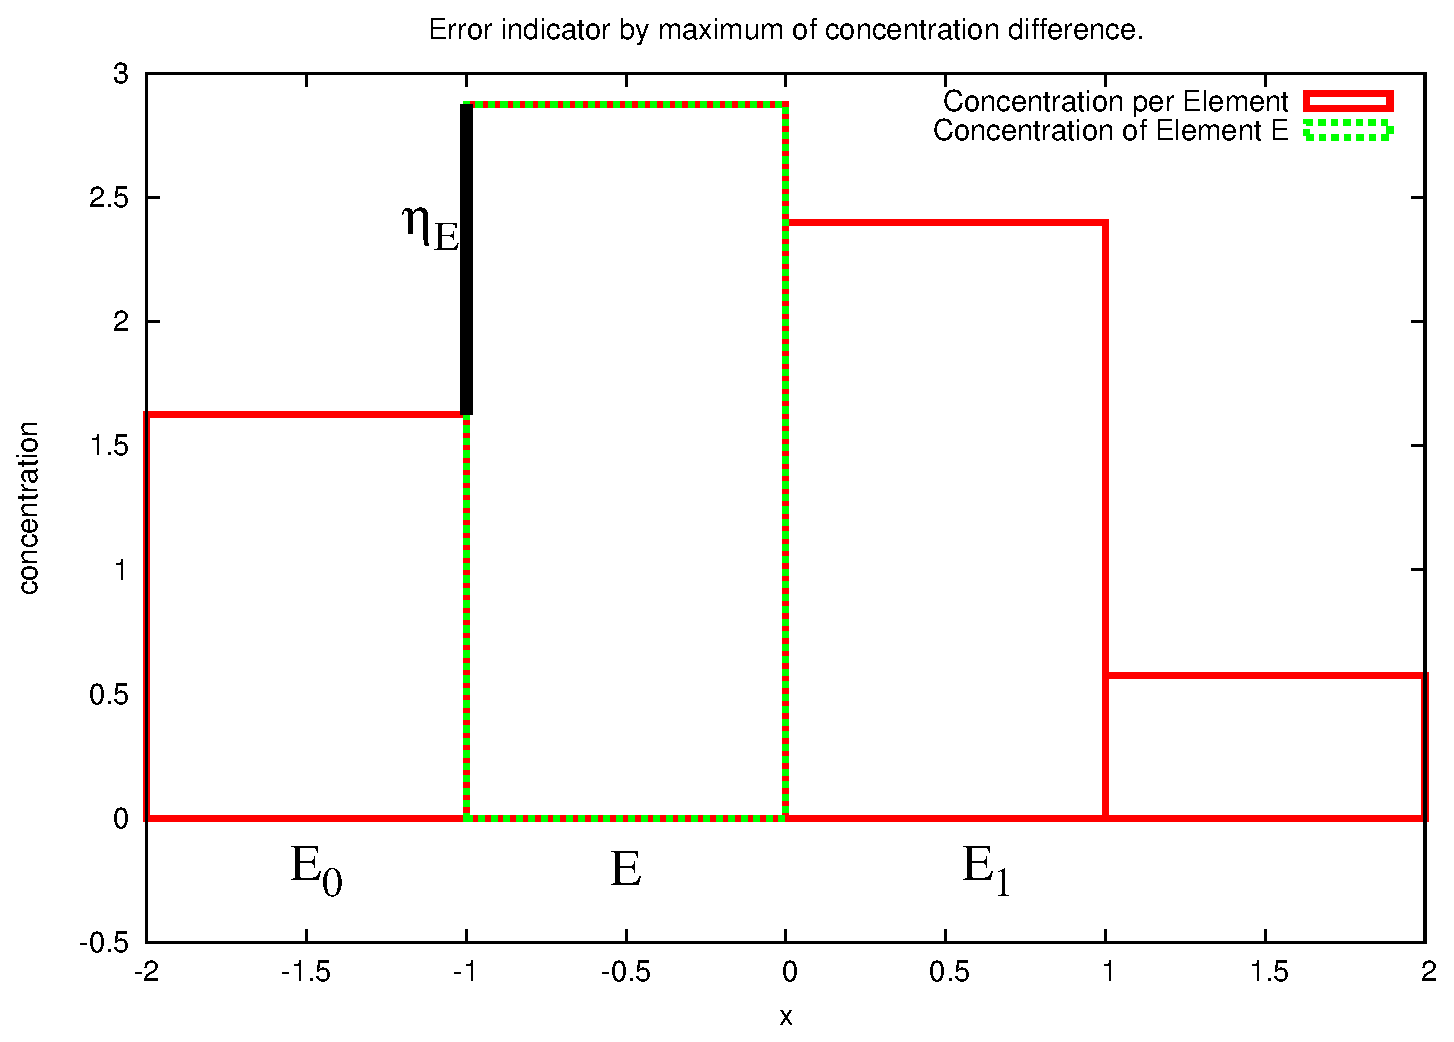
\includegraphics[width=0.95\textwidth]{EPS/adaptivity/errind_maxconc}
      \end{center}
    \end{minipage}
  \end{center}
\end{frame}

\begin{frame}
  \frametitle<presentation>{What is adaptivity all about?}
  There are two main ways to increase the local resolution:
  \begin{itemize}
    \item Use smaller elements at the points of interest (\emph{$h$-Refinement})
    \item Increase the polynomial degree of the elements (\emph{$p$-Refinement})
  \end{itemize}

  The two approaches can be combined, of course. This is called $hp$-Refinement.

  We will focus on $h$-Refinement.

\end{frame}

\subsection{$h$-Refinement}

\begin{frame}
  \frametitle<presentation>{$h$-Refinement}
  In \emph{$h$-Refinement}, the mesh size $h$ is decreased in areas that need a high resolution. To achieve this, the cells in the affected areas are replaced by cells with a \emph{smaller diameter}.

  There are several different strategies for finding a suitable refinement. Things to consider are e.g.~the \emph{construction effort} and the \emph{quality} of the resulting cells (anisotropy, inner angles, distance between nodes\ldots).

  We will have a look at
  \begin{itemize}
    \item Edge Bisection
    \item Red-Green Refinement
  \end{itemize}
\end{frame}

\subsubsection*{Bisection}

\begin{frame}
  \frametitle<presentation>{Edge Bisection}
  \begin{center}
    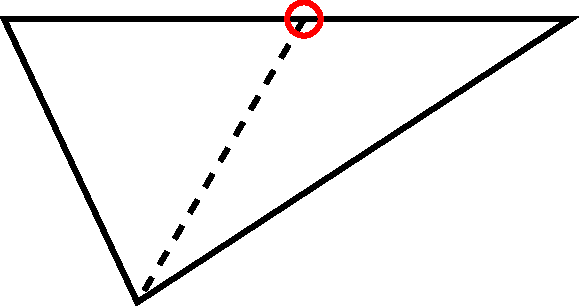
\includegraphics[width=0.45\textwidth]{EPS/adaptivity/bisection}
  \end{center}
  \begin{itemize}
    \item each element is split into two
    \item choice of edge is important: \newline
      bisection of the shortest edge will lead to poor mesh quality
    \item used in \emph{AlbertaGrid}
  \end{itemize}
\end{frame}

\subsubsection*{Red-Green Refinement}

\begin{frame}
  \frametitle<presentation>{Red-Green Refinement}
  \begin{center}
    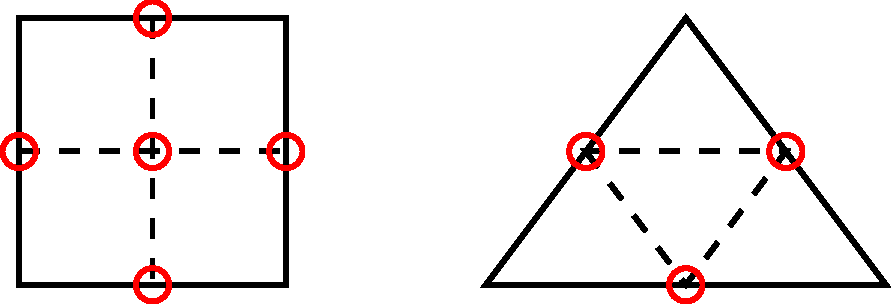
\includegraphics[width=0.45\textwidth]{EPS/adaptivity/redgreen}
  \end{center}
  \begin{itemize}
    \item is also called \emph{regular refinement}
    \item used in \emph{ALUGrid} and \emph{UGGrid}
    \item simplicial case (triangle, tetrahedron): \newline
      new vertices are placed in the center of edges,
    \item quadrilateral, hexadron: new vertices are placed in the center of edges, sides and volumes
    \item results are \emph{similar} (i.e.~congruent up to scaling)
  \end{itemize}
\end{frame}

\begin{frame}
  \frametitle{Regular Refinement of Elements}

  \begin{center}
    \begin{minipage}{0.8\textwidth}
      \begin{center}
        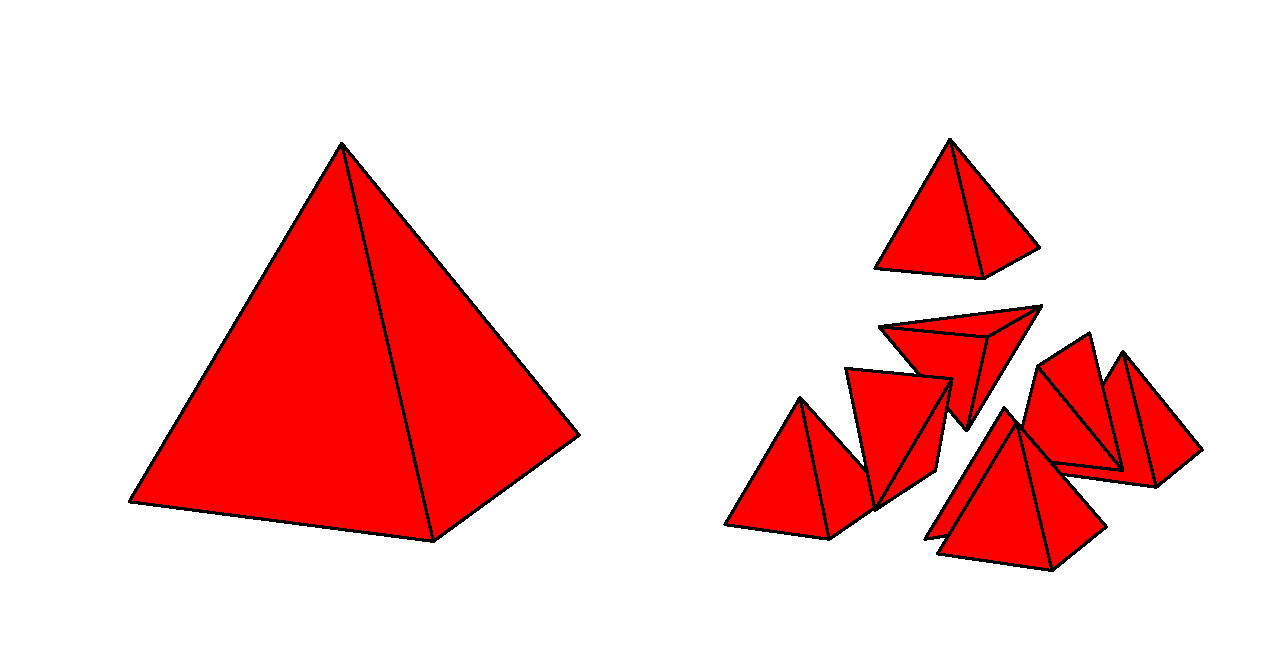
\includegraphics[width=0.45\linewidth]{EPS/adaptivity/refinetet}
        \hfill
        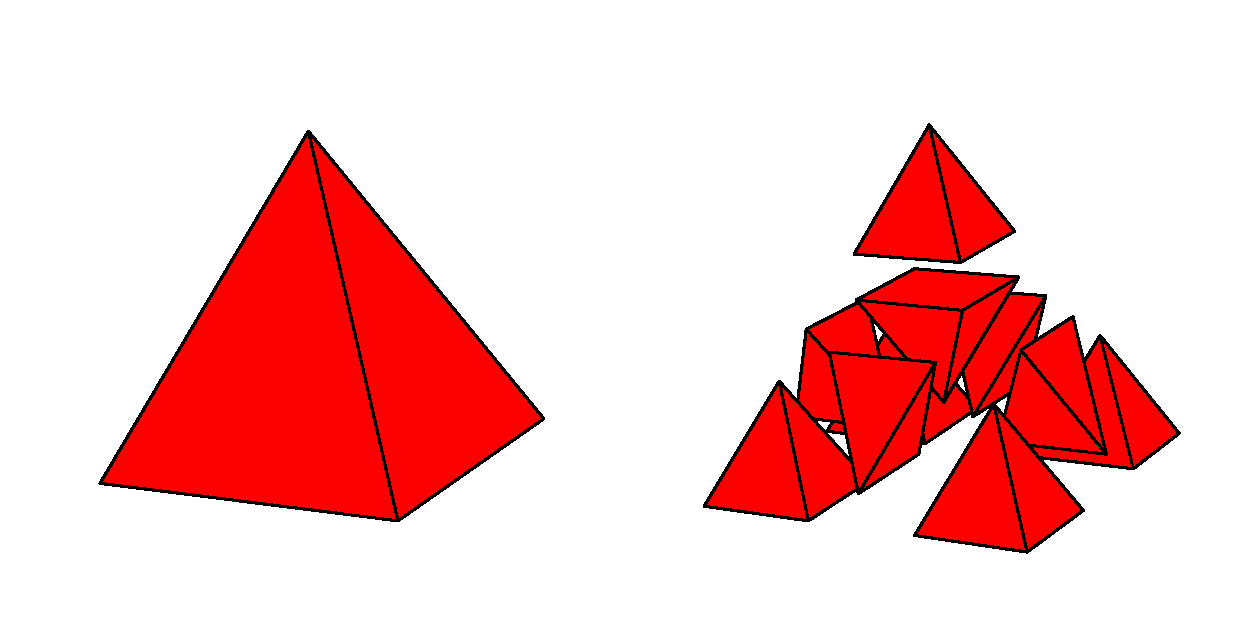
\includegraphics[width=0.45\linewidth]{EPS/adaptivity/refinepyr}\\

        Tetrahedron \hspace*{3cm} Pyramid
      \end{center}
      \vspace{0.5cm}
      \begin{center}
        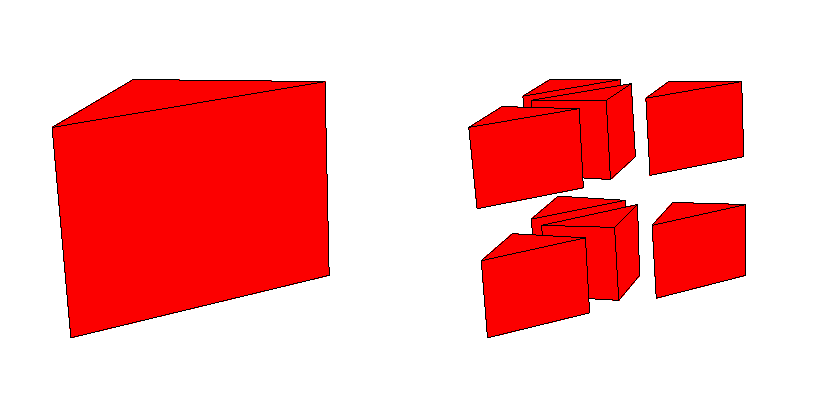
\includegraphics[width=0.45\linewidth]{EPS/adaptivity/refinepri}
        \hfill
        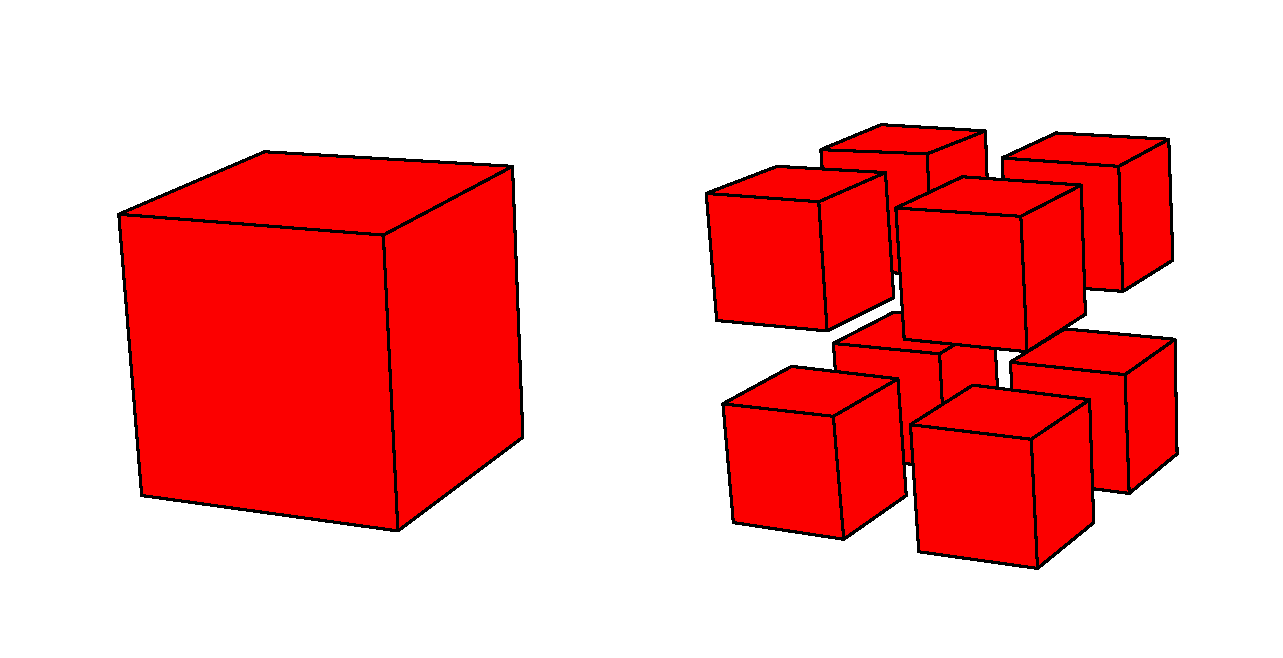
\includegraphics[width=0.45\linewidth]{EPS/adaptivity/refinehex}

        Prism \hspace*{3cm} Hexahedron
      \end{center}
    \end{minipage}
  \end{center}
\end{frame}


\subsubsection*{Hanging nodes}

\begin{frame}
  \frametitle<presentation>{Hanging Nodes}

  \begin{center}
    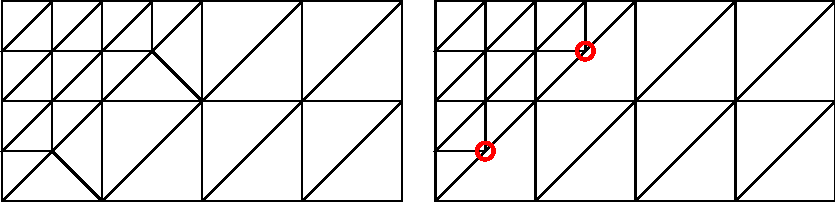
\includegraphics[width=0.95\textwidth]{EPS/adaptivity/hanging}
  \end{center}

  Local refinement may lead to so called hanging nodes, sitting on the edge of a coarser element.

  In contrast to regular nodes, hanging nodes may not be true degrees of freedom, e.g.~in the case of a conforming ansatz space.
\end{frame}

\begin{frame}
  \frametitle<presentation>{Hanging Nodes}
  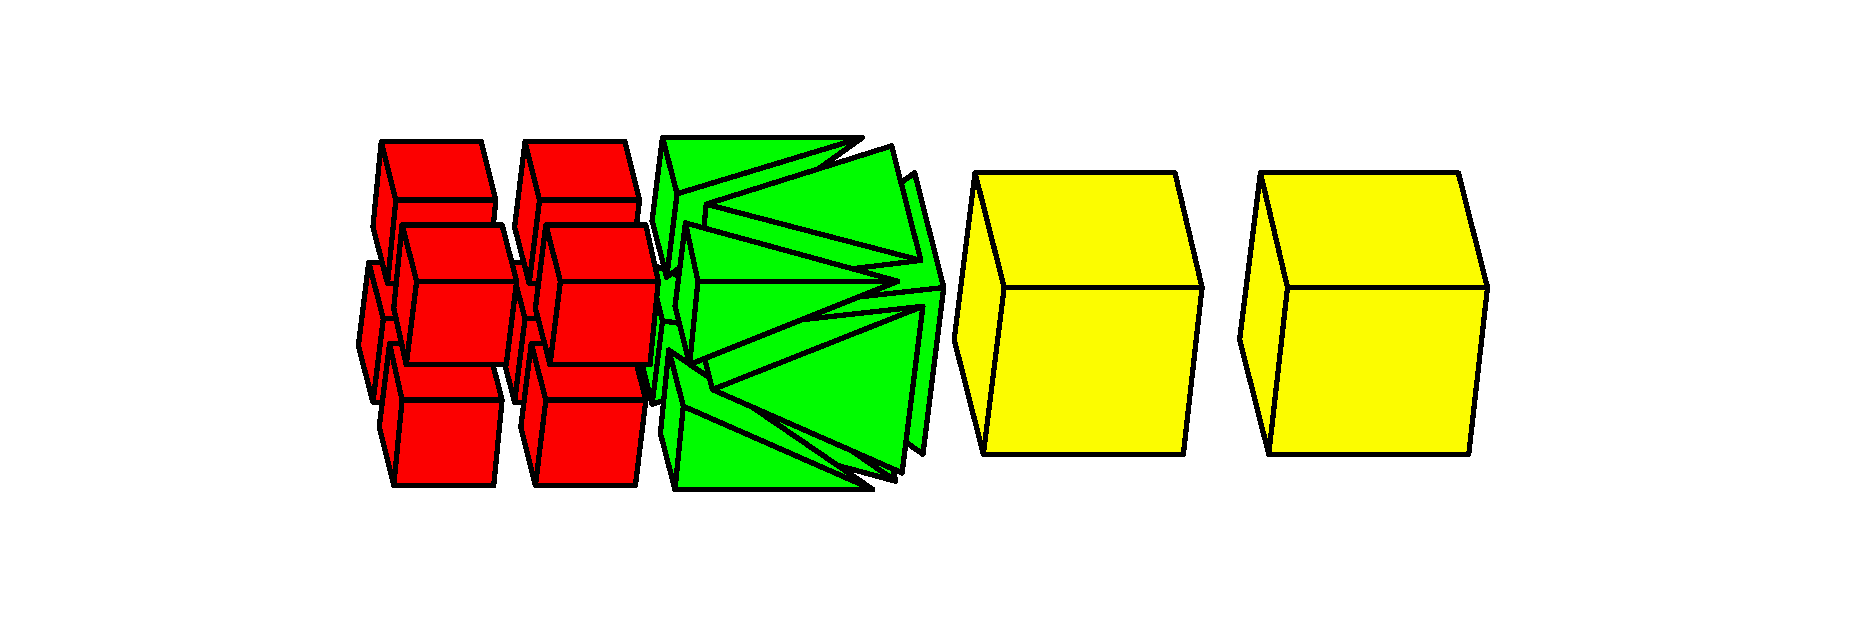
\includegraphics[width=\linewidth]{EPS/adaptivity/hexclosurenew}

  \begin{block}{Conforming Closure}
    \begin{itemize}
      \item Regular (red), irregular (green) and copy (yellow) refinements
      \item Conforming closure for each possible situation ($2^{19}$ cases for hexahedra)
      \item no iteration process necessary $\rightarrow$ well suited for parallelization
    \end{itemize}
  \end{block}
\end{frame}

\subsection{Adaptivity in DUNE}

\subsubsection*{Workflow}

\begin{frame}<presentation>
  \frametitle{Grid Access: Viewing vs. Modification}
  The DUNE Grid interface follows the \emph{View-only} Concept.
  \pause
  \only<presentation>{\vfill}
  \structure{View-Only Concept}
  \begin{itemize}
    \item Views offer (read-only) access to the data
      \begin{itemize}
        \item Read-only access to grid entities allow the consequent use of const.
        \item Access to entities is only through iterators for a
          certain view. 
          \begin{itemize}
            \item[$\Rightarrow$] \emph{This allows on-the-fly implementations.}
          \end{itemize}
      \end{itemize}
    \item  Data can only be modified in the primal container \emph{(the Grid)}
  \end{itemize}
  \pause
  \only<presentation>{\vfill}
  \structure{Modification Methods:}
  \begin{itemize}
    \item  Global Refinement

    \item  \textcolor{red}{Local Refinement \& Adaptation}

    \item  Load Balancing
  \end{itemize}
\end{frame}

\begin{frame}
  \frametitle<presentation>{Marking Elements} 

  {\bf First phase:} {Marking of elements}
  \begin{itemize}
    \item The method\newline
      \lstinline{bool mark (int refCount, const Codim<0>::Entity& e)}\newline
      is used to mark an entity \lstinline{e} for 
      \begin{itemize}
        \item refinement (refCount $> 0$) or 
        \item coarsening (refCount $< 0$)
        \item neither (refCount = 0).
      \end{itemize}
      It returns \lstinline{true} if the counter has been updated
      successfully.
    \item  Calling the method\newline
      \lstinline{int getMark (const Codim<0>::Entity& e) const}\newline
      returns the current refinement counter of an entity.
  \end{itemize}
\end{frame}

\begin{frame}
  \frametitle<presentation>{Grid Adaptation} 

  {\bf Second phase:} {Grid modification}
  \begin{enumerate}
    \item Call the grid's method \lstinline{grid.preAdapt()}. This method \emph{prepares}
      the grid for adaptation. It returns \lstinline{true} if at least one entity was
      marked for coarsening.

      \pause

    \item If \lstinline{grid.preAdapt()} returned \lstinline{true}, any data associated with
      entities that might be coarsened during the following adaptation
      cycle has to be \emph{projected} to the father entities.

      \pause

    \item Call \lstinline{grid.adapt()}. The grid is \emph{modified} according to the
      adaptation marks.

      \pause

    \item If \lstinline{grid.adapt()} returned \lstinline{true}, new entities were created.
      Existing data must be \emph{prolongated} to newly created entities.

      \pause

    \item Call \lstinline{grid.postAdapt()} to \emph{clean up} refinement markers.
  \end{enumerate}

  \pause

  As the data management is the user's responsibility, he or she has to
  take care of restriction and prolongation of data attached to the grid. 
  This is possible using the persistent index maps 
  i.\,e., \lstinline{LocalIdSet} and \lstinline{GlobalIdSet}.
\end{frame}

\begin{frame}
  \frametitle{Data Transfer between Grids}

  The {\sc Dune} \lstinline{Entity<0>} class provides two methods, which are
  needed during the grid modification phase for solution transfer:
  \begin{itemize}
    \item The method\newline
      \lstinline{bool mightVanish () const}\newline
      returns \lstinline{true} if the entity {\bf \emph{might}} be removed when
      \lstinline{grid.adapt()} is called. 

      \pause

    \item The method\newline
      \lstinline{bool isNew () const}\newline
      returns \lstinline{true} if the entity was newly generated in the
      grid modification process, otherwise \lstinline{false}.
  \end{itemize}

  \pause

  \begin{block}{\emph{Note:}}
    Both methods may only be called between \lstinline{grid.preAdapt()}
    and \lstinline{grid.postAdapt()}.
  \end{block}

\end{frame}

\begin{frame}
  \frametitle{Solution Transfer during Adaptation I}  

  \begin{center}
    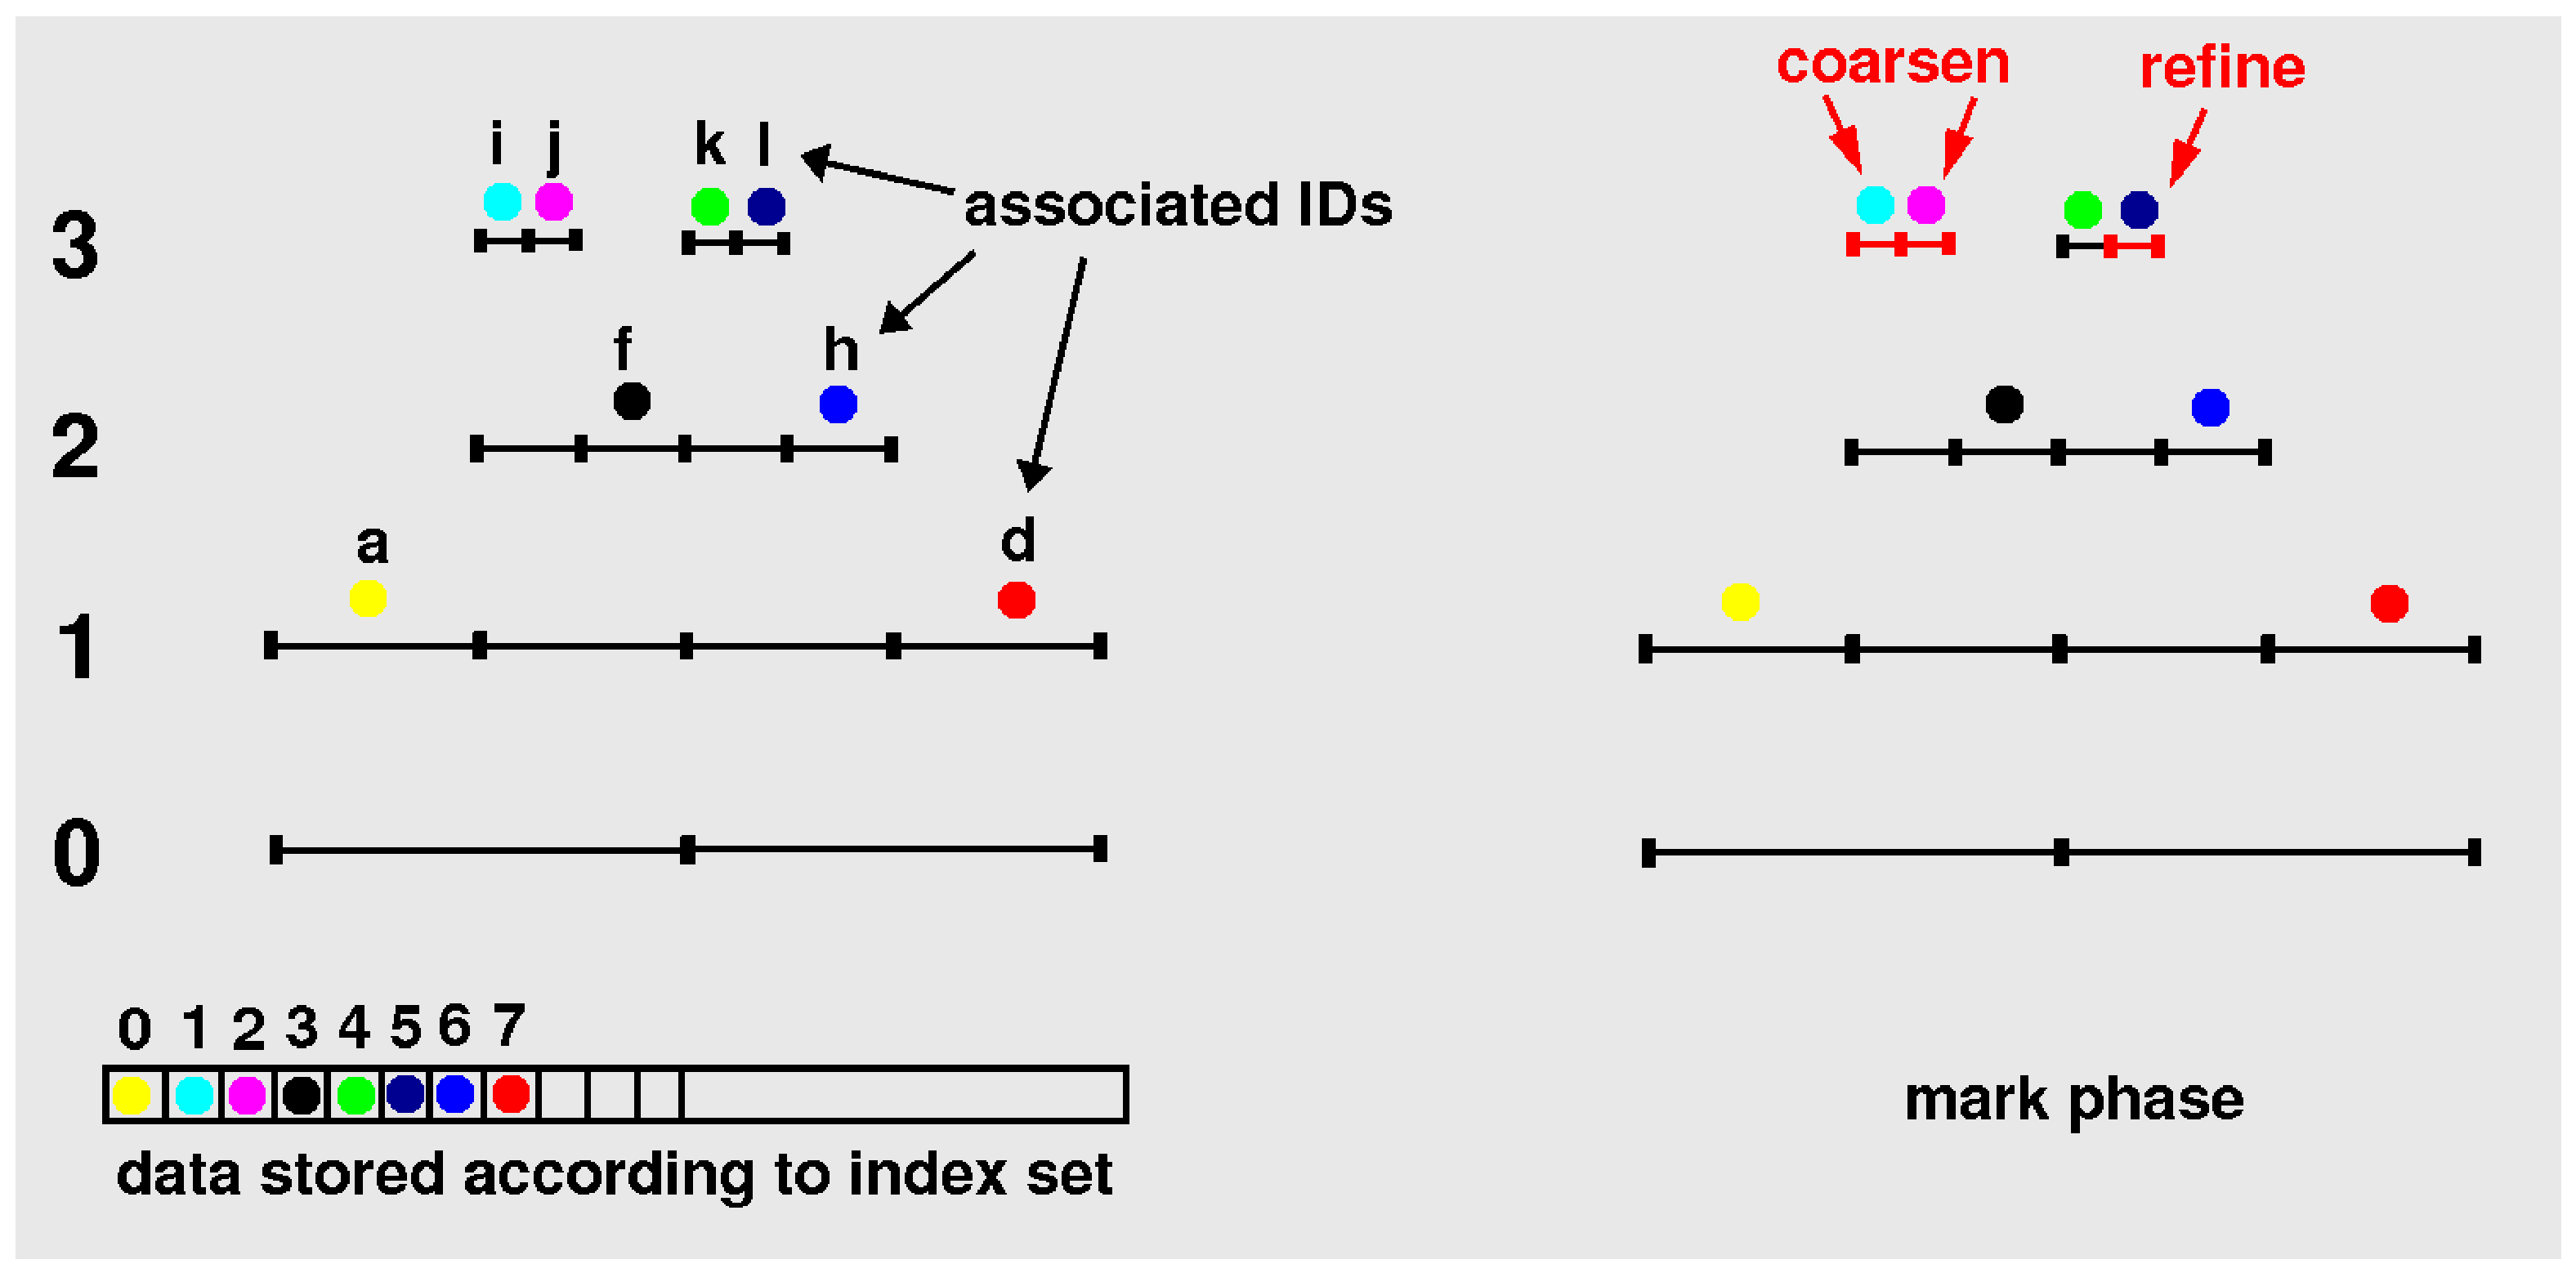
\includegraphics[width=0.9\textwidth]{EPS/adaptivity/hadapt}
  \end{center}

\end{frame}

\begin{frame}
  \frametitle{Solution Transfer during Adaptation II}  

  \begin{center}
    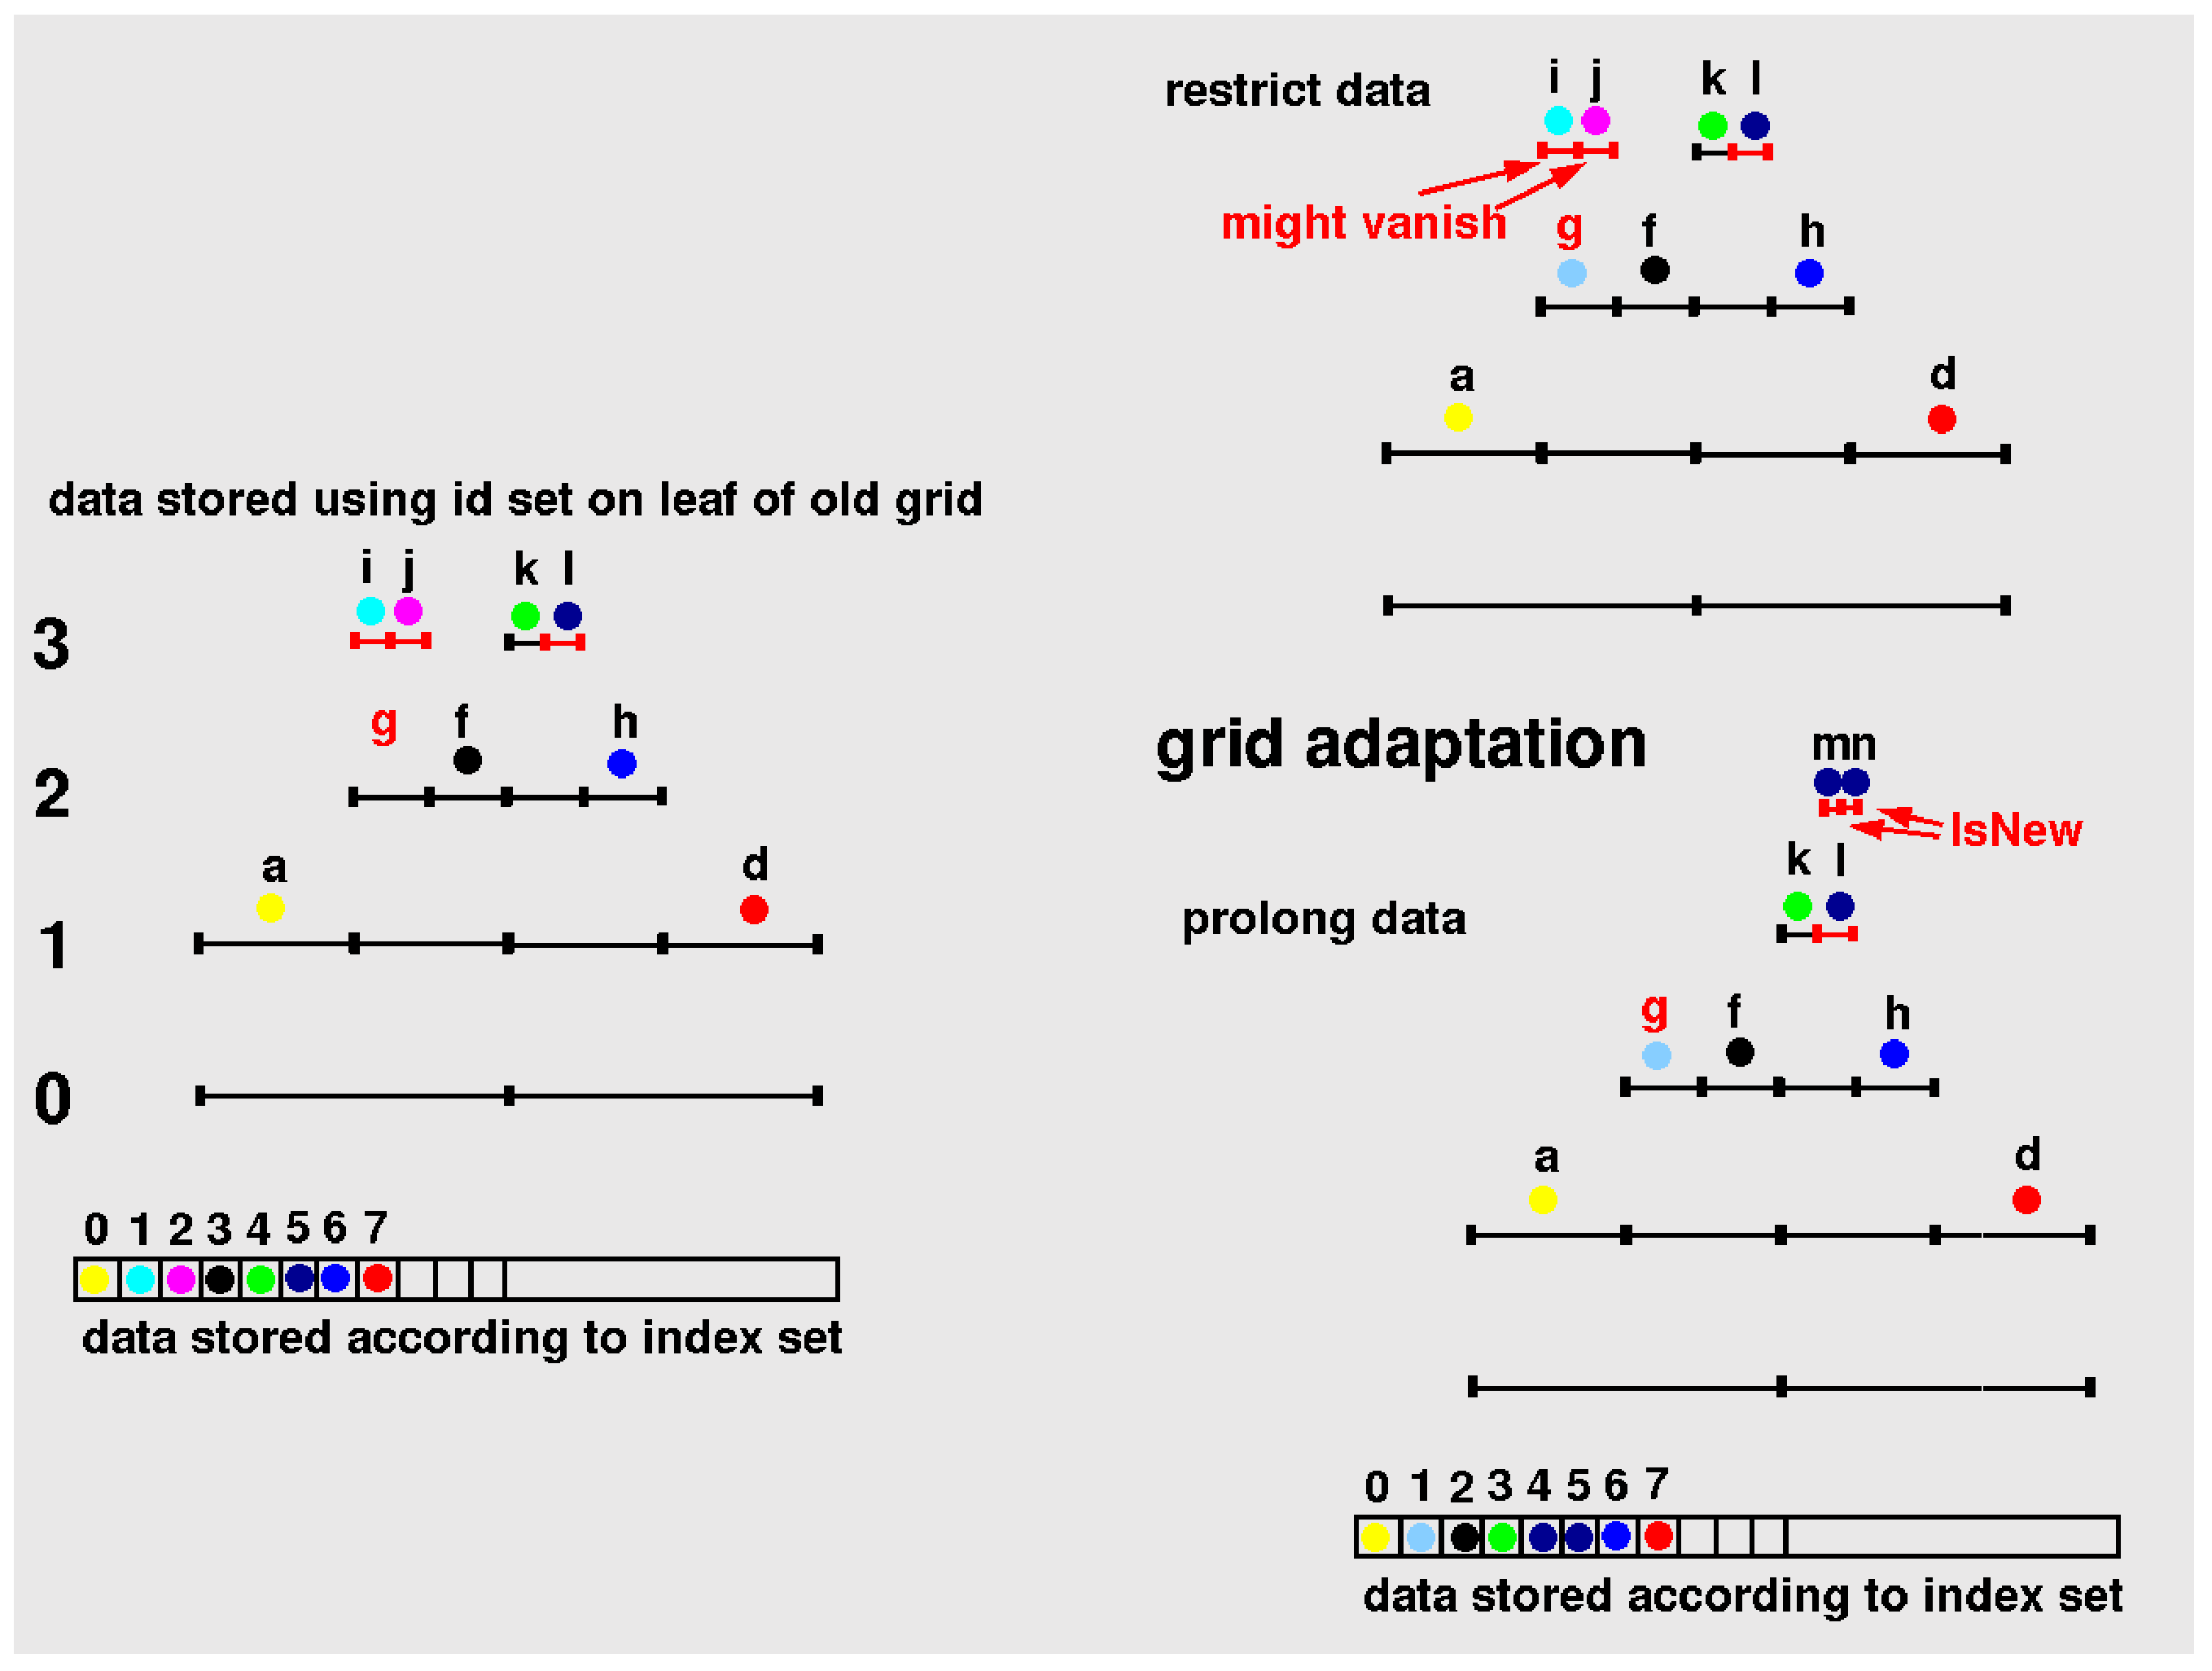
\includegraphics[width=0.8\textwidth]{EPS/adaptivity/hadapt1}
  \end{center}

\end{frame}

\begin{frame}
  \frametitle<presentation>{Summary}
  \begin{block}{\emph{Summary}}
    \begin{enumerate}
      \item mark the appropriate cells
      \item backup/project your data (preAdapt, mightVanish-Flags)
      \item adapt the grid proper
      \item restore/interpolate your data (postAdapt, isNew-Flags)
    \end{enumerate}
  \end{block}
  \pause
  \begin{block}{\emph{But:}}
    PDELab does all of this for you!
  \end{block}
\end{frame}

\subsubsection*{The Grids and their abilities}

\paragraph{YaspGrid}

\begin{frame}
  \frametitle<presentation>{YaspGrid}
  \begin{center}
    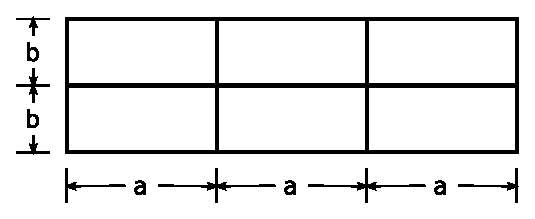
\includegraphics{EPS/adaptivity/cartesian}
  \end{center}
  \begin{block}{\emph{YaspGrid}}
    is used in most of the examples.

    It is a \emph{Cartesian} grid, i.e.~a tensor grid with equidistant spacing in each dimension, and therefore \emph{cannot} be locally refined.
  \end{block}
\end{frame}

\paragraph{Other Grids}

\begin{frame}
  \frametitle<presentation>{Other Grids}

  \begin{block}{\emph{AlbertaGrid}}
    The grid manager of the ALBERTA toolbox. 
    ALBERTA is sequential code and supports simplicial grids in one, two, and 
    three space dimensions with \emph{bisection refinement}.

  \end{block}

  \begin{block}{\emph{ALUGrid}}
    A parallel 2d and 3d hexahedral and tetrahedral grid with \emph{nonconforming regular refinement} and dynamic load balancing.

  \end{block}

  \begin{block}{\emph{UGGrid}}
    The grid manager of the UG toolbox.
    UG provides a parallel grid manager in two and three space dimensions 
    that supports hybrid meshes with local \emph{red--green or nonconforming 
    refinement}.


  \end{block}
\end{frame}


\subsection{Adaptivity in PDELab}

\subsubsection*{Refinement loop}

The adaptive refinement loop in listing 20 starts at the line 53. For $i=0$, our
PDE is solved (line 64) on the base grid level. The solution is stored in the
vector of degrees of freedom $u$ (line 31). Afterwards, we will compute
a local error indicator $\eta$ (lines 78-79) for the solution $u$.
Based on this information, we will be able to decide which grid elements
should be marked for refinement (or coarsening) in the next step.
For this decision, we offer two different strategies: element fraction or error fraction.

Example: If you choose a refinement fraction $\alpha=0.2$, this means in the
case of element fraction that the top $20\%$ of all
elements in terms of local error will be refined, or, in the case of error
fraction, the contribution of all refined cells to the total error is $20\%$.

After the grid function space and the solution are also adapted on the grid,
note that the Dirichlet boundary constraints need to be
re-applied on the adapted solution vector $u$ (line 104).


\subsubsection*{Error indicator $\eta$}
$\eta$ is supposed to be cell-wise constant. Therefore, we setup a grid function space using the $P_0$
finite element. Since we need to traverse the whole grid once, we can
simply use the infra\/struture provided by Dune::PDELab::GridOperator.
All you need to contribute yourself is a local operator (line 49) that
implements the evaluation of the local error indicator.
It is highly dependent upon the actual differential equation and on your
choice. A simple example is given in \lstinline{example07_error_indicator.hh}.
It uses large jumps in the normal component of the gradient across element
boundaries as an indicator.



\subsubsection*{Refinement/coarsening fraction and threshold}
\begin{block}{Function call}
  \lstinline{element_fraction( eta, alpha, beta, eta_alpha, eta_beta, verbose  );}\\
  or: \lstinline{error_fraction( eta, alpha, beta, eta_alpha, eta_beta, verbose );}
\end{block}

\begin{tabular}{l|lll}
  parameter   & meaning                                          & type    &  \\
\hline
  eta         & DOF vector containing the local error indicators & U0      & input \\
  alpha       & refinement fraction                              & double  & input  \\
  beta        & coarsening fraction                              & double  & input  \\
  eta\_alpha  & refinement threshold                             & double  & output \\
  beta\_alpha & coarsening threshold                             & double  & output \\
  verbose     & verbosity flag                                   & int     & input  \\
\end{tabular}



\subsubsection*{Marking the grid for local adaptation}
\begin{block}{Function call}
  \lstinline{mark_grid( grid, eta, eta_alpha, eta_beta );}
\end{block}

\begin{tabular}{l|lll}
  parameter   & meaning                                          & type    &  \\
  \hline
  grid        & the grid object                                  & Grid    & input+output \\
  eta         & DOF vector containing the local error indicators & U0      & input \\
  eta\_alpha  & refinement threshold                             & double  & input \\
  beta\_alpha & coarsening threshold                             & double  & input \\
\end{tabular}


\subsubsection*{Adapting the grid and adjusting the solution vector}
\begin{block}{Function call}
  \lstinline{adapt_grid( grid, gfs, u );}
\end{block}

\begin{tabular}{l|lll}
  parameter   & meaning                                          & type    &  \\
  \hline
  grid        & the grid object                                  & Grid    & input+output \\
  gfs         & the grid function space                          & GFS     & input+output \\
  u           & DOF vector containing the solution of the PDE    & U       & input+output \\
\end{tabular}




\subsection{Example 7}

\begin{frame}
  \frametitle{Example 7 Overview}

  Example 7 applies an adaptation scheme to the problem of Example 2, generating the series of solutions seen in the beginning of this section.

  It consists of the files
  \begin{itemize}
    \item \lstinline{example07.cc} -- main program.
    \item \lstinline{example07_adaptivity.hh} -- driver using adaptivity.
    \item \lstinline{example07_error_indicator.hh} -- local indicators.
    \item \lstinline{example02_(...).hh} -- problem definition as before.
  \end{itemize}
\end{frame}

\begin{frame}<presentation>[fragile,allowframebreaks,allowdisplaybreaks]
  \frametitle<presentation>{Adaptive Driver}
  \framesubtitle<presentation>{File \texttt{src/course-examples/example07\_adaptivity.hh}}
  \lstinputlisting[basicstyle=\tiny,numbers=left, 
  numberstyle=\tiny, numbersep=2pt]{../../src/course-examples/example07_adaptivity.hh}
\end{frame}

\mode<article>{
\begin{Lst}[File src/course-examples/example07\_adaptivity.hh] \mbox
  \nopagebreak
  \lstinputlisting[basicstyle=\scriptsize,numbers=left, 
  numberstyle=\tiny, numbersep=2pt]{../../src/course-examples/example07_adaptivity.hh}
\end{Lst}}

